\documentclass{article}
\usepackage{graphicx}
\usepackage{gensymb}
\title{Aerodynamics Activity}
\author{Micaiah Smith-Pierce, Yohannes Kasseya}
\date{18-Feb-2017}
\begin{document}
\maketitle
\begin{itemize}
\item{}
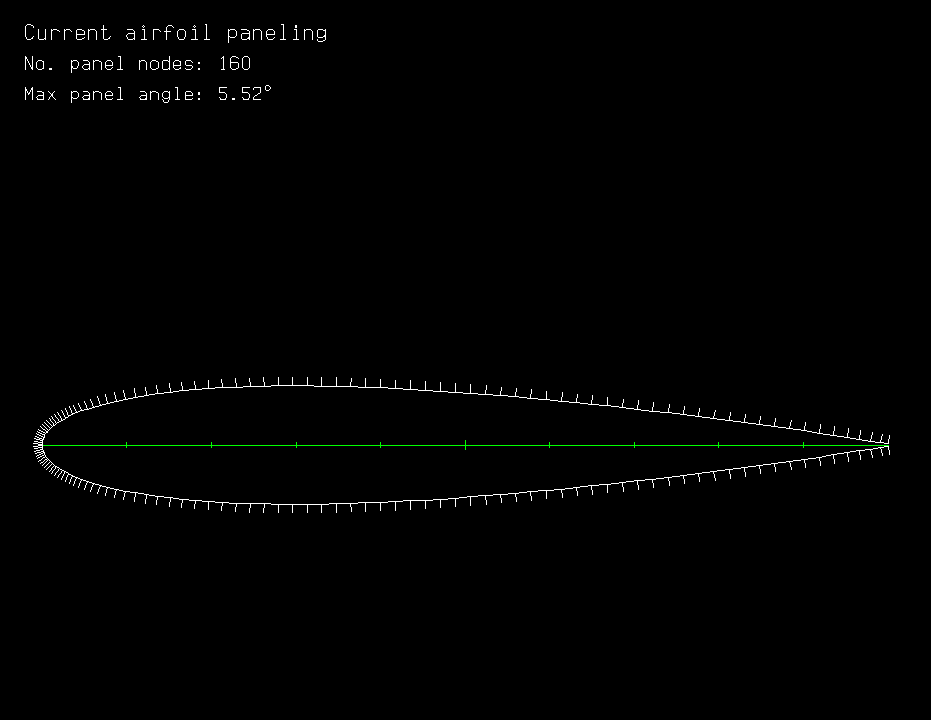
\includegraphics[width = 10cm]{coordinate_plot.png}

\item{The program clearly predicts stall.  At approximately $\alpha = 12$ for $Re = 10^5$ and $\alpha = 15$ for $Re = 10^6$ $C_L$ drops sharply,
and shortly after that, $C_D$ rises dramatically.  $C_M$ is also affected.}

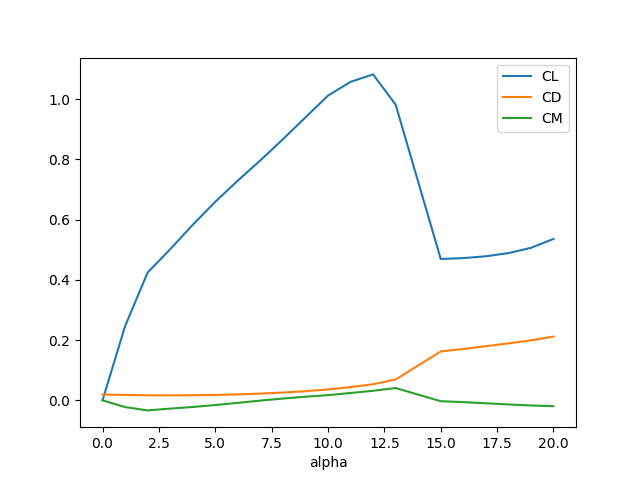
\includegraphics[width = 10cm]{reE5.png}

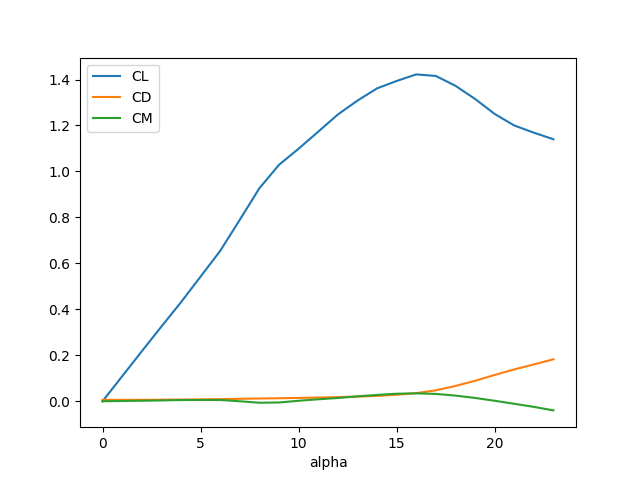
\includegraphics[width = 10cm]{reE6.png}

\item{The data set was restricted to the linear regime and a linear fit calculated using the \verb|polyfit| function from Python's \verb|numpy|
library.  In order to calculate the ${C_L}_\alpha$ quoted here slope of said best fit line was converted from degrees to radians.}
\begin{itemize}
\item{$Re = 10^5 : {C_L}_\alpha = 4.70$}
\item{$Re = 10^6 : {C_L}_\alpha = 5.40$}
\end{itemize}

\item{For one thing, at every point along the chord, the pressure coefficient on the upper surface is less than on the lower surface. 
In addition, the difference is largest near the leading edge and smallest near the trailing edge.}
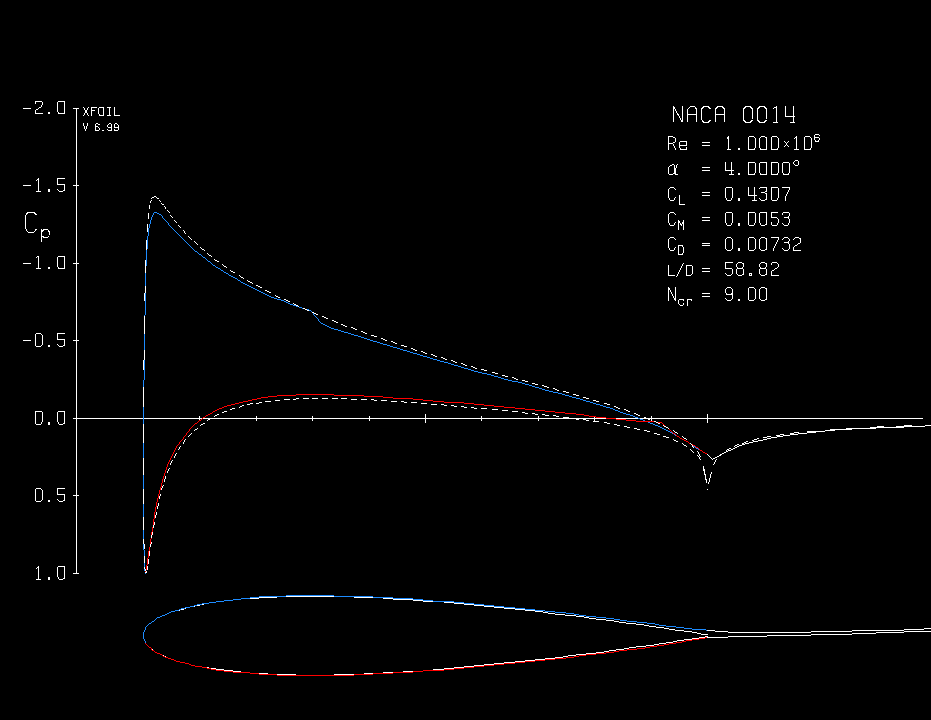
\includegraphics[width = 10cm]{alfa_4.png}

\item{The distribution is considerably different.  The $C_P$ near the trailing edge is approximately zero instead of being positive.
 In general, the fact that the $C_P$ deviates heavily from the inviscid prediction (dashed line) indicates stall.  However, the airfoil
does not appear to be completely stalled, since the $C_P$ is close to the inviscid prediction near the leading edge, and the $C_L$ is still
near ${C_L}_{max}$.}

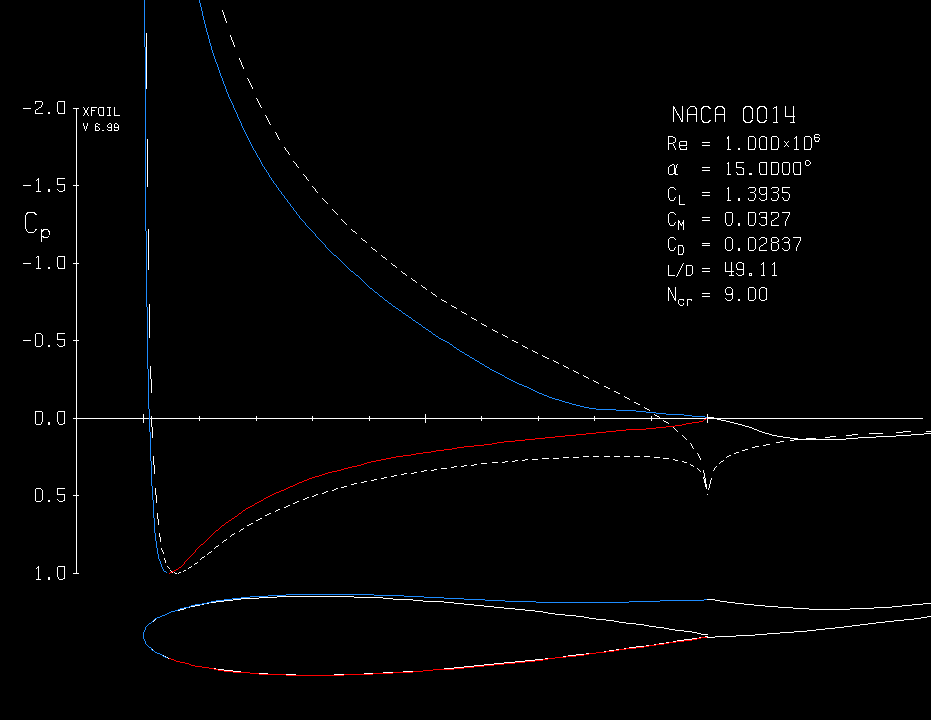
\includegraphics[width = 10cm]{alfa_15.png}

\item{Using the spreadsheet from the atmosphere assignment, it was calculated that at 2500m, $\rho = 0.95 kg/m^3$.  Since calculating the
Reynolds number would require knowing the velocity which we are endeavoring to obtain, the value of ${C_D}_0$ was initialized using 
$Re = 10^6$.  An iterative process was used to find the actual value of $Re$ and ${C_D}_0$.}


\item{Let the speed for minimum drag be denoted $V_{min}$.  The equation below was used to calculate it:
\[ (\frac{W^2}{S^2 \rho^2 {C_D}_0 \pi AR e})^\frac{1}{4} \]}
\item{The following equations were also used:
\[C_L = \frac{2 W}{\rho {V_{min}}^2 S} \]
\[ {C_D}_i = \frac{{C_L}^2}{\pi AR e} \]
\[ D = ({C_D}_0 + {C_D}_i)\frac{1}{2} \rho {V_{min}}^2 S \]}

\item{$V_{min}$ was calculated using the equation above, and used to find a more accurate value of $Re$.  The value $\mu = 17.29*10^-6 Pa*s$
was used (the temperature from the atmosphere assignment was passed as a parameter to the following online calculator:

\verb|www.engineeringtoolbox.com/air-absolute-kinematic-viscosity-d_601.html|).  Subsequently, the value of $Re$ obtained was used to calculate a
more accurate value of ${C_D}_0$, and so on, until it was discovered that:
\[V_{min} = 52 m/s\]
\[Re = 5*10^6\]}

\item{Using the equation given in part (7), the lift curve slope, in degrees, was found to be 0.1071.  We then have $C_L = 1.01$ and $\alpha =
9.46\degree$.}

\item{In case it was not intended that we would calculate our own Reynolds number, $Re = 10^5$ was used to obtain the following values:}

\begin{tabular}{l | l}
\hline
${C_D}_0$ & 0.01899\\ \hline
$V_{min}$ & $39 m/s$\\ \hline
$C_L$ & 0.60\\ \hline
${C_L}_\alpha$ & 0.11\\ \hline
$\alpha$ & $5.59\degree$\\ \hline
\end{tabular}

\end{itemize}
\end{document}

